\documentclass[a4paper,12pt]{article}
\usepackage[toc,page]{appendix}
\usepackage{listings}
\usepackage{hyperref}
\usepackage{graphicx}
\usepackage[skip=0pt]{caption}
\usepackage{multicol}
\usepackage{float}
\usepackage[margin=1in]{geometry}

\begin{document}

\renewcommand{\thelstlisting}{\thesection-\arabic{lstlisting}}
\renewcommand{\thefigure}{\arabic{section}-\arabic{figure}}
\setlength{\floatsep}{0pt plus 2pt minus 2pt}
%\setlength{\intextsep}{0pt plus 2pt minus 2pt}
%\setlength{\textfloatsep}{0pt plus 2pt minus 2pt}

\title{Introduction to Digital Libraries Assignment \#3}
\date{March 31, 2015}
\author{James Tate II}
\maketitle

\section{Introduction}

\section{Methodology}

\subsection{Subsection Name}
%\begin{lstlisting}[basicstyle=\ttfamily,caption={Downloading Tweets}]
%    ./download_tweets.py
%\end{lstlisting}

\section{Statistics}

%\begin{figure}[H]
%    \centering
%    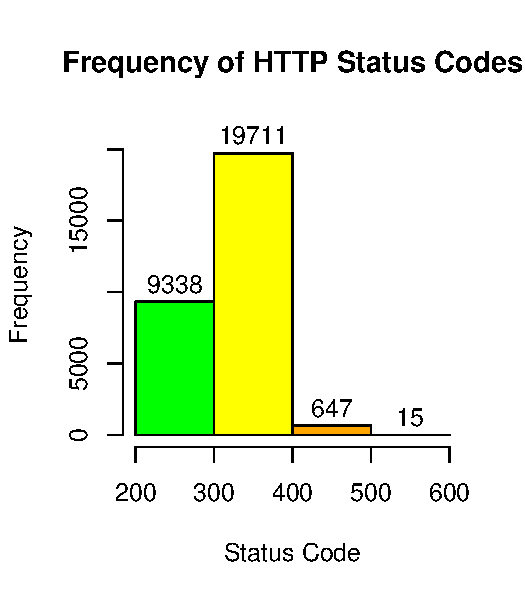
\includegraphics{stats/http_status_codes.pdf}
%    \caption{Frequency of HTTP status codes in histogram by sequential category.
%}
%\end{figure}

\clearpage
\begin{appendices}

\section{Streaming API Filter Keywords}
These keywords were selected arbitrarily. Keywords were added to the list until the streaming
API seemed to pull tweets at a strong, consistent rate.
\begin{multicols}{3}
\begin{itemize}
    \item python
    \item fsf
    \item foss
    \item coding
    \item programming
    \item fedora
    \item rhel
    \item dovetail
    \item woodworking
    \item blizzard
    \item snowstorm
    \item colorado
    \item virginia
    \item internet
    \item library
    \item libraries
    \item json
    \item lemonade
    \item woodchuck
    \item iasip
    \item league
    \item awesomenaut
    \item tf2
\end{itemize}
\end{multicols}

\end{appendices}




\begin{thebibliography}{9}
\bibitem{rfc2616}
    R. Fielding, et. al.,
    \emph{Hypertext Transfer Protocol -- HTTP/1.1}.
    \url{https://www.ietf.org/rfc/rfc2616.txt}
    June 1999.


\end{thebibliography}

\end{document}
